% !TEX root = MAIN.tex

\section{SEMuS}

\subsection{Software static architecture}

\begin{figure}[tb]
  \centering
  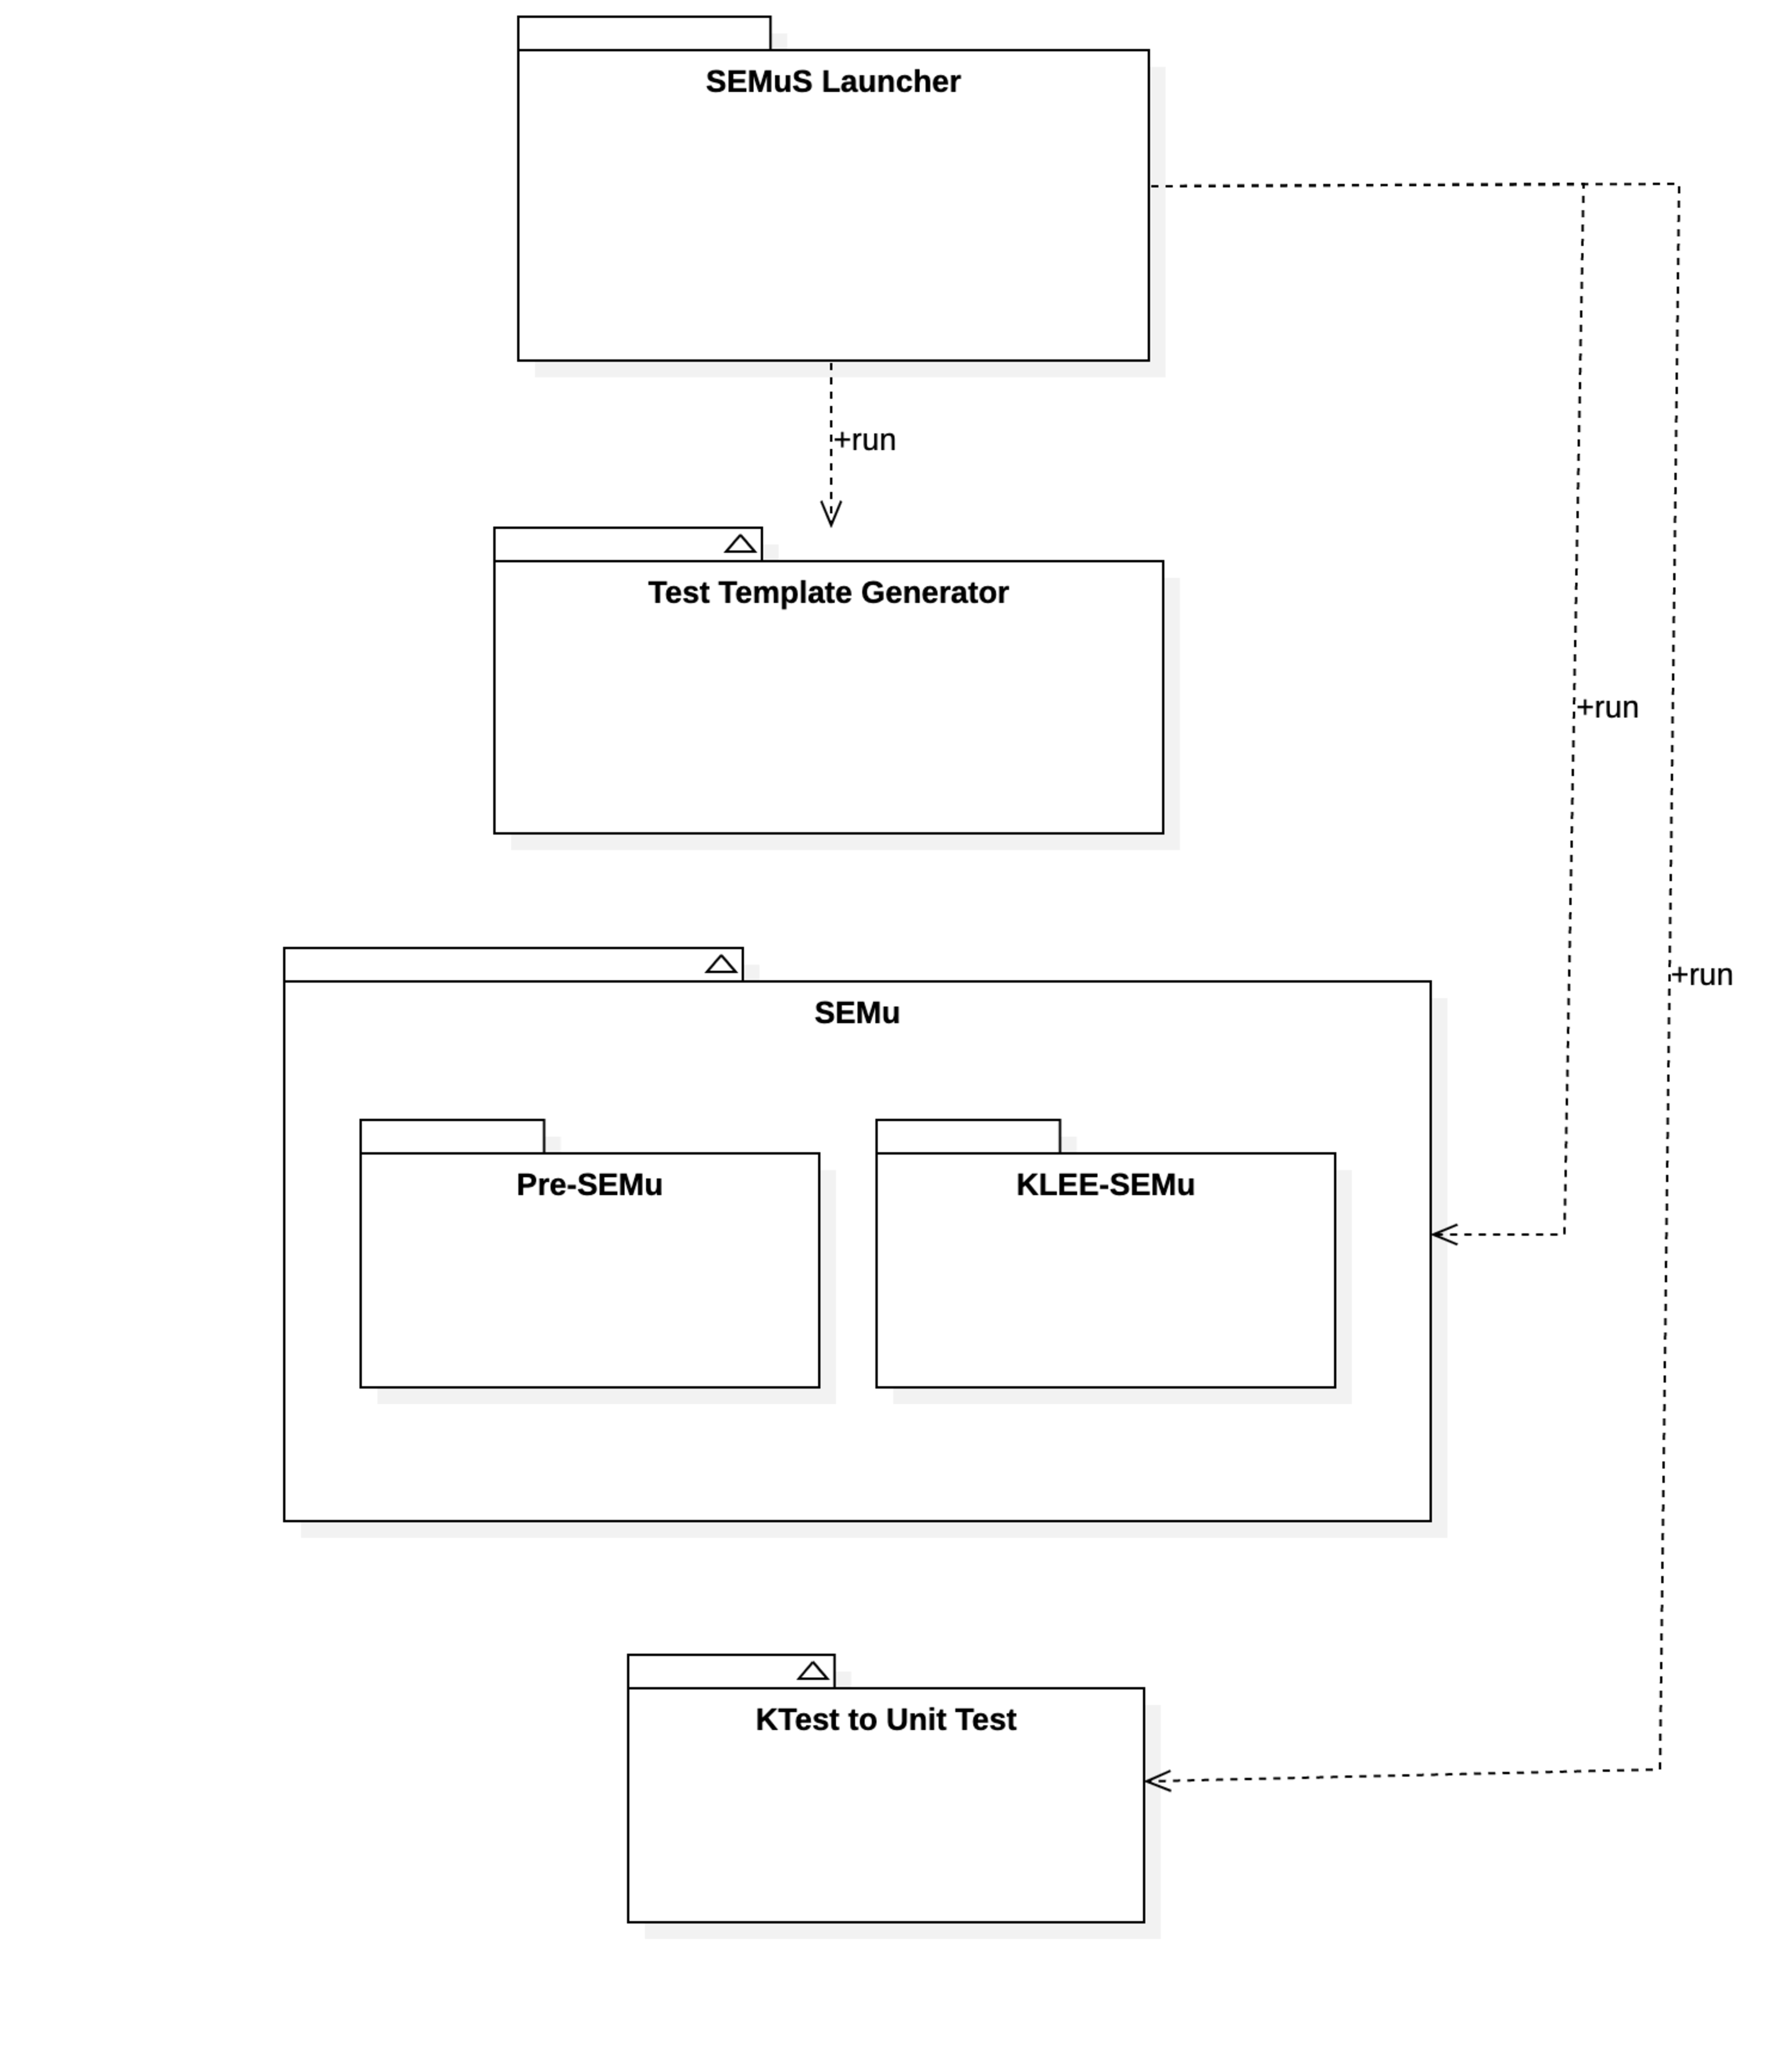
\includegraphics[width=0.6\textwidth]{images/semus-arch-sdd}
      \caption{UML Architecture diagram of SEMuS.}
      \label{fig:architecture_diagram_semus}
\end{figure}

The architecture of the code-driven test suite augmentation toolset (i.e., SEMuS) is drafted in Figure~\ref{fig:architecture_diagram_semus}. The architecture diagram relies on UML package diagram notation.

As specified in Figure~\ref{fig:architecture_diagram_semus}, the architecture of the toolset is divided into three packages:(1) the \emph{Test Template Generator}, (2) the \emph{SEMu}, and (3) the \emph{KTest to Unit Test}. The diagram also includes the entry point of the toolset, which is the \emph{SEMuS Launcher}.

The package \emph{Test Template Generator} implements the features concerning (1) the parsing of the SUT source code, and (2) the generation of test templates for each SUT function.

The package \emph{SEMu} implements the features regarding (1) the generation of the meta mutant, (2) the compilation of the meta mutant, (3) the compilation of the test template, and (4) the invocation of the underlying test generation tool (i.e., KLEE).

The package \emph{KTest to Unit Test} implements the features concerning (1) the parsing of KLEE's output, and (2) the conversion of KLEE tests to C unit test cases.

\subsubsection{Source Code Structure}

SEMuS is delivered as a compressed archive containing a set of source files and an installer. In the following, there is a brief description of the archive's structure once uncompressed:

\begin{itemize}
  \item \texttt{SEMuS/}
    \begin{itemize}
      \item \texttt{underlying\_test\_generation/}: contains the source files of the component that invokes KLEE-SEMu.
      \item \texttt{pre\_semu/}: contains the source files of the component that prepares the meta-mutant file to be processed by KLEE-SEMu.
      \item \texttt{ktest\_to\_unittest/}: contains the source files that implements the component that parses the output of KLEE (i.e., KLEE tests) and converts it to readable C unit test cases.
      \item \texttt{case\_studies/}: contains the configuration files, SUT source codes, and SEMuS launchers for the case studies ASN.1 and MLFS.
      \begin{itemize}
        \item \texttt{scripts/}: contains the configuration files and launchers of the case study.
        \item \texttt{util\_codes/}: folder containing the generated test templates for the case study.
        \item \texttt{WORKSPACE/}: folder containing the SUT source code and list of live mutants.
      \end{itemize}
      \item \texttt{Dockerfile}: text document file that contains all the commands necessary to build a Docker container with all the dependencies of SEMuS.
      \item \texttt{cd\_semu\_docker.sh}: bash script that automates the execution of the toolset through the use of Docker.
      \item \texttt{install\_requirements.sh}: build script that installs SEMuS' requirements.
      \item \texttt{requirements.txt}: list of Python packages to be parsed by \texttt{install\_requirements.sh}.
    \end{itemize}
\end{itemize}

\subsection{Software components design}
\label{sec:component:design:semus}

\begin{figure}[tb]
  \centering
  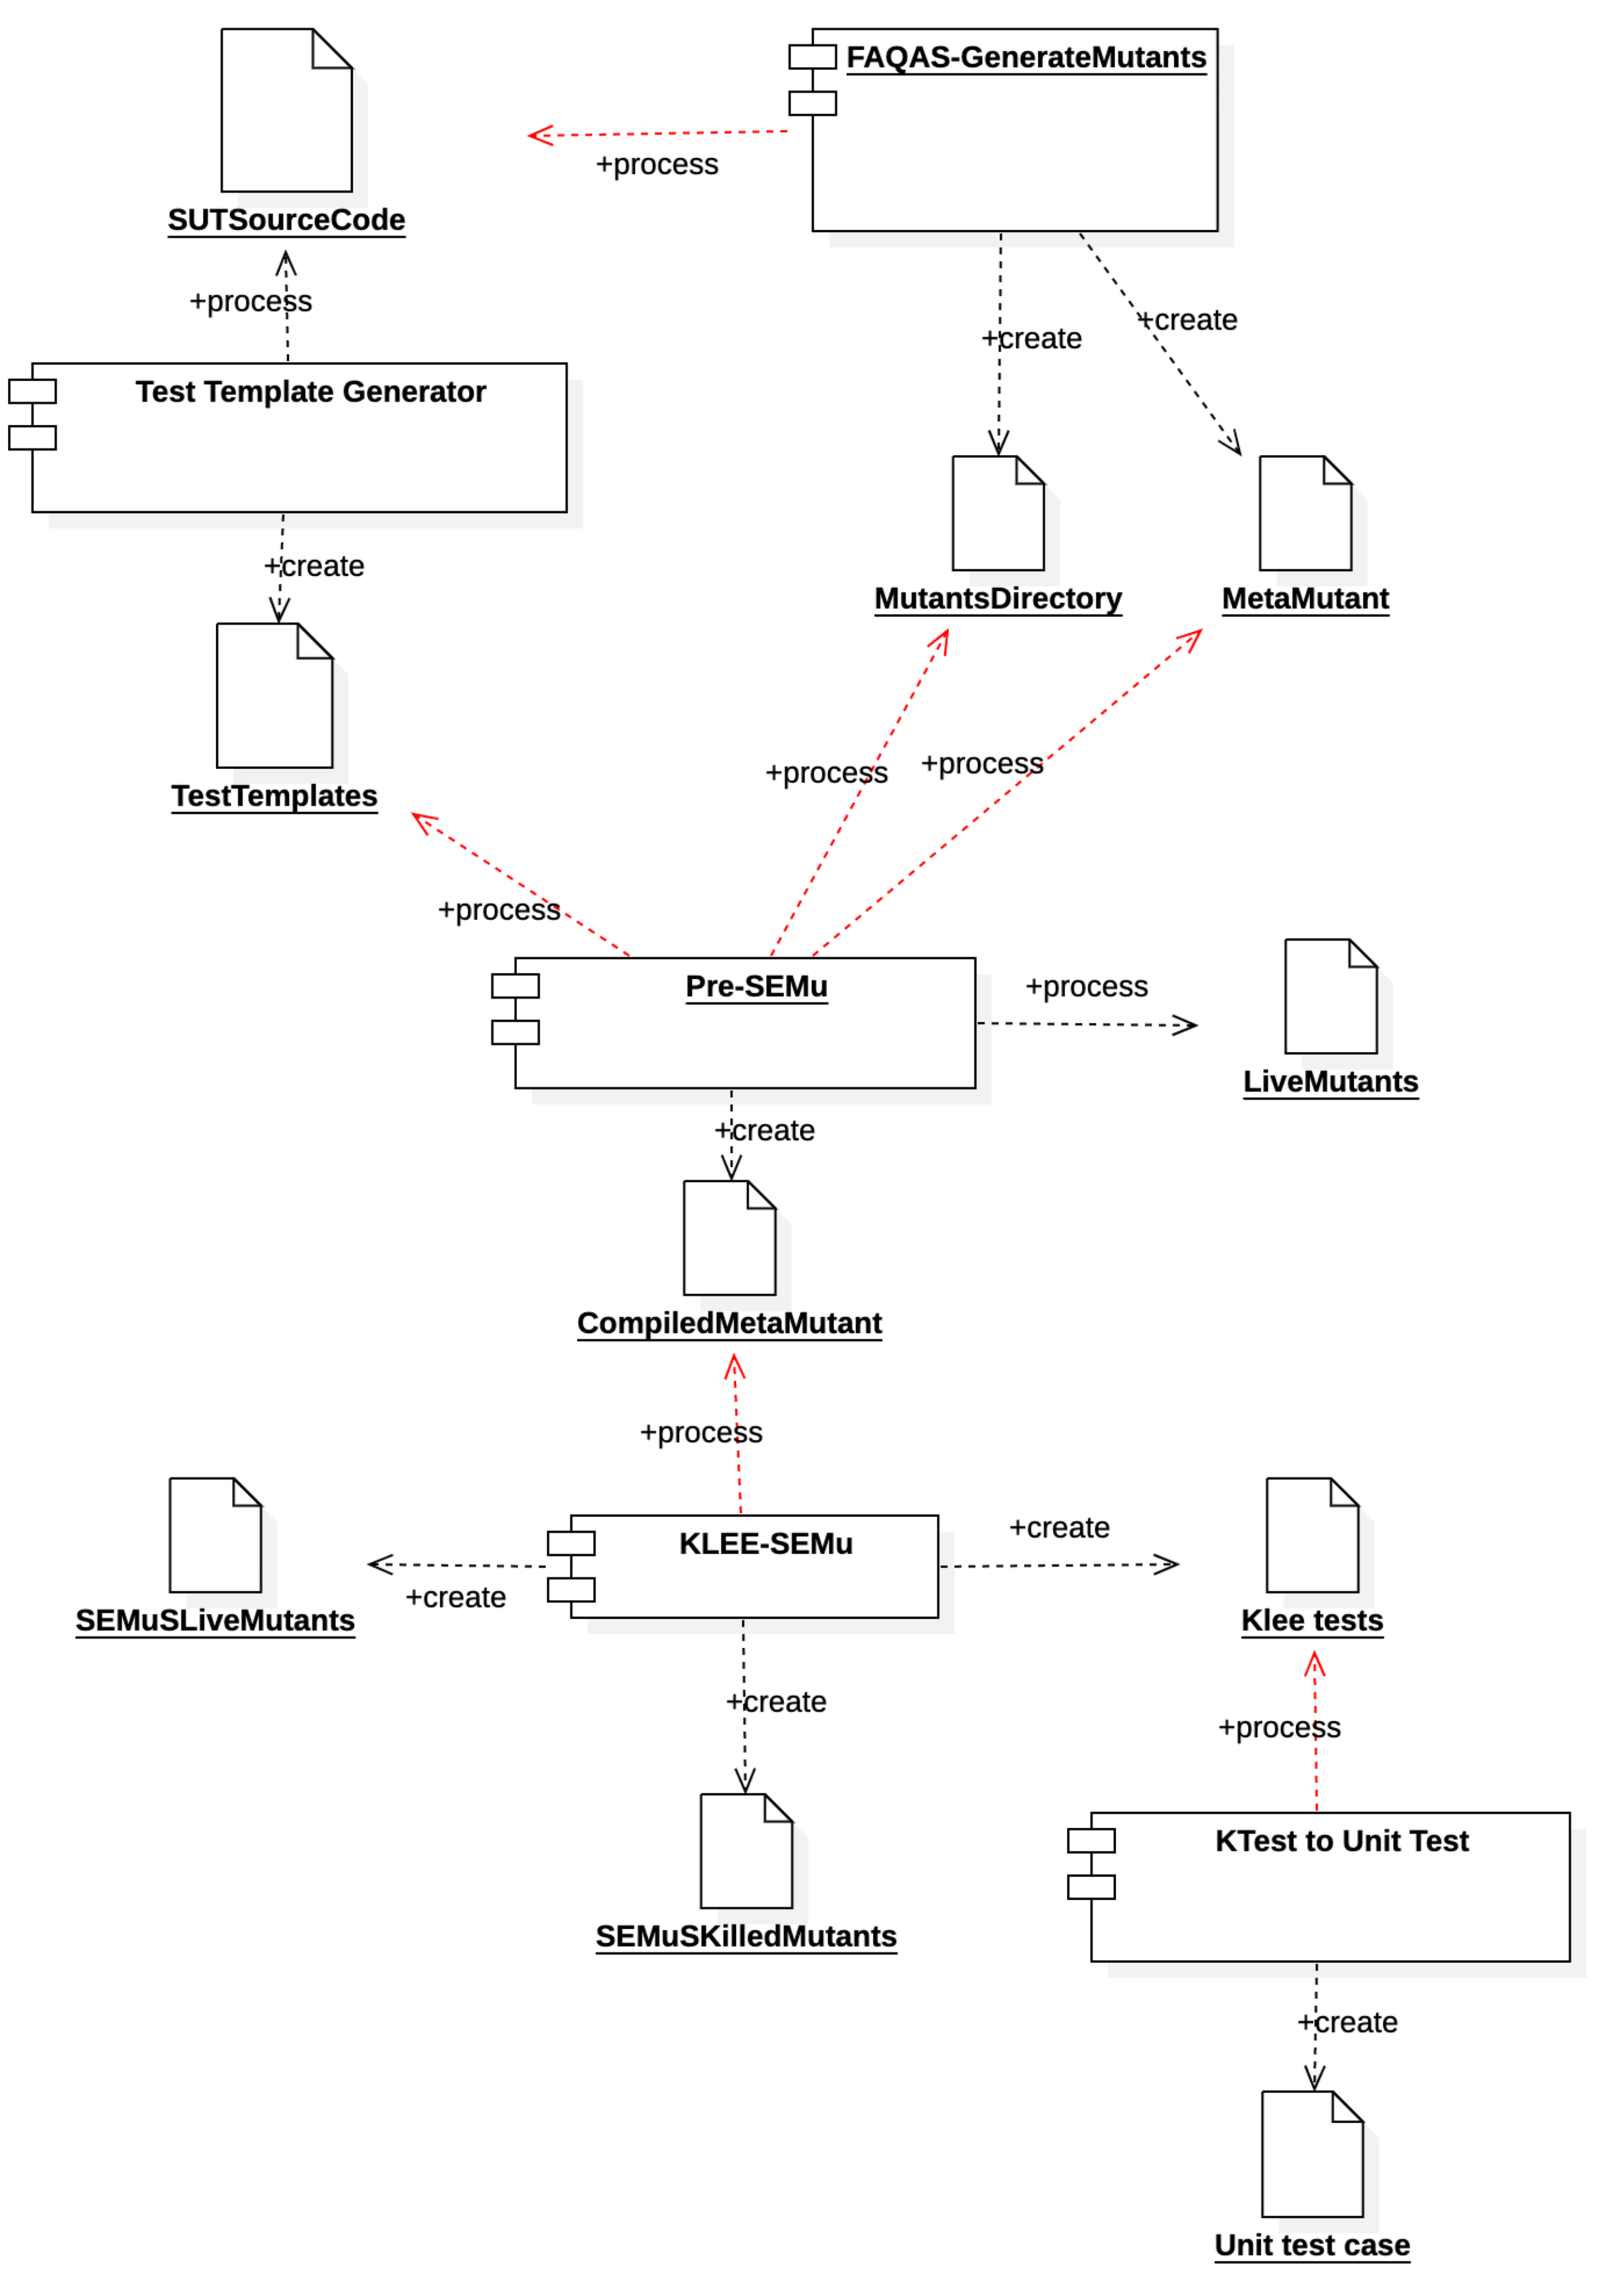
\includegraphics[width=0.7\textwidth]{images/semus-component.pdf}
      \caption{UML Component diagram of the code-driven test suite augmentation toolset (SEMuS).}
      \label{fig:component_diagram_semus}
\end{figure}


The components of SEMuS are drafted in Figure~\ref{fig:component_diagram_semus}. Figure~\ref{fig:component_diagram_semus} relies on UML component diagram notation.

As shown in Figure~\ref{fig:component_diagram_semus}, the software is composed by the following components:

\begin{itemize}
  \item \emph{Test Template Generator}: this component processes the SUT source code and generates the files \emph{TestTemplates}. The information produces by the component is mainly processed by \emph{Pre-SEMu}.
  \begin{itemize}
    \item \emph{TestTemplates}: test template (i.e., C source file) that contains the wrapping main function for driving the test generation for a specific SUT function.
  \end{itemize}
  \item \emph{FAQAS-GenerateMutants}: this component originally belongs to MASS (see Section~\ref{sec:component:design}), it processes the SUT source code and creates the file \emph{MetaMutant}, and a \emph{MutantsDirectory} including the source code for every mutant targeting a specific source code.
  \begin{itemize}
    \item \emph{MetaMutant}: Source code (i.e., C file) that includes all the mutants for a specific source; every mutated statement is controlled by a switch statement that decides the mutant to be activated during testing.
  \end{itemize}
  \item \emph{Pre-SEMu}: this component processes the files \emph{TestTemplates}, \emph{MetaMutant}, the \emph{MutantsDirectory}, and creates the \emph{CompiledMetaMutant} file. The information produced by the component is processed mainly by the underlying test generation tool (i.e., KLEE-SEMu).
  \begin{itemize}
    \item \emph{CompiledMetaMutant}: LLVM bytecode consisting of the compiled code of the \emph{MetaMutant} and the \emph{TestTemplates} for a specific source file. This file follows the format required by KLEE-SEMu, and KLEE in general.
  \end{itemize}
  \item \emph{KLEE-SEMu}: this component processes the \emph{CompiledMetaMutant} generated by \emph{Pre-SEMu}, and creates the files \emph{KLEE tests}, \emph{SEMuSKilledMutants} and \emph{SEMuSLiveMutants}. The component configures and invokes the underlying test generation tool with the adequate parameters and configurations.
  \begin{itemize}
    \item \emph{KLEE tests}: set of inputs that kill the mutants for a specific source. The inputs are created following the KLEE format for test cases.
    \item \emph{SEMuSKilledMutants}: list of mutants identifiers for which KLEE-SEMu did generate at least one test input.
    \item \emph{SEMuSLiveMutants}: list of mutants identifiers for which KLEE-SEMu did not generate any test input.
  \end{itemize}
  \item \emph{KTest to Unit Test}: this component processes the \emph{KLEE tests} generated by \emph{KLEE-SEMu}, and creates the files \emph{Unit test case}.
  \begin{itemize}
    \item \emph{Unit test case}: readable C unit test case containing an invocation to the SUT function, where the parameters' values are derived from \emph{KLEE-SEMu} output.
  \end{itemize}
\end{itemize}


\subsection{Software behavior}


% The activity \emph{Execute FAQAS-CompileAndExecuteMutants} in Figure~\ref{fig:process:codeDriven:augmentation} concerns the execution of the program \emph{FAQAS-GenerateTestGenerationScaffolding}.
\TODO{Control flow arrows are missing on the SEMUs actor side}
\begin{figure}[tb]
  \centering
  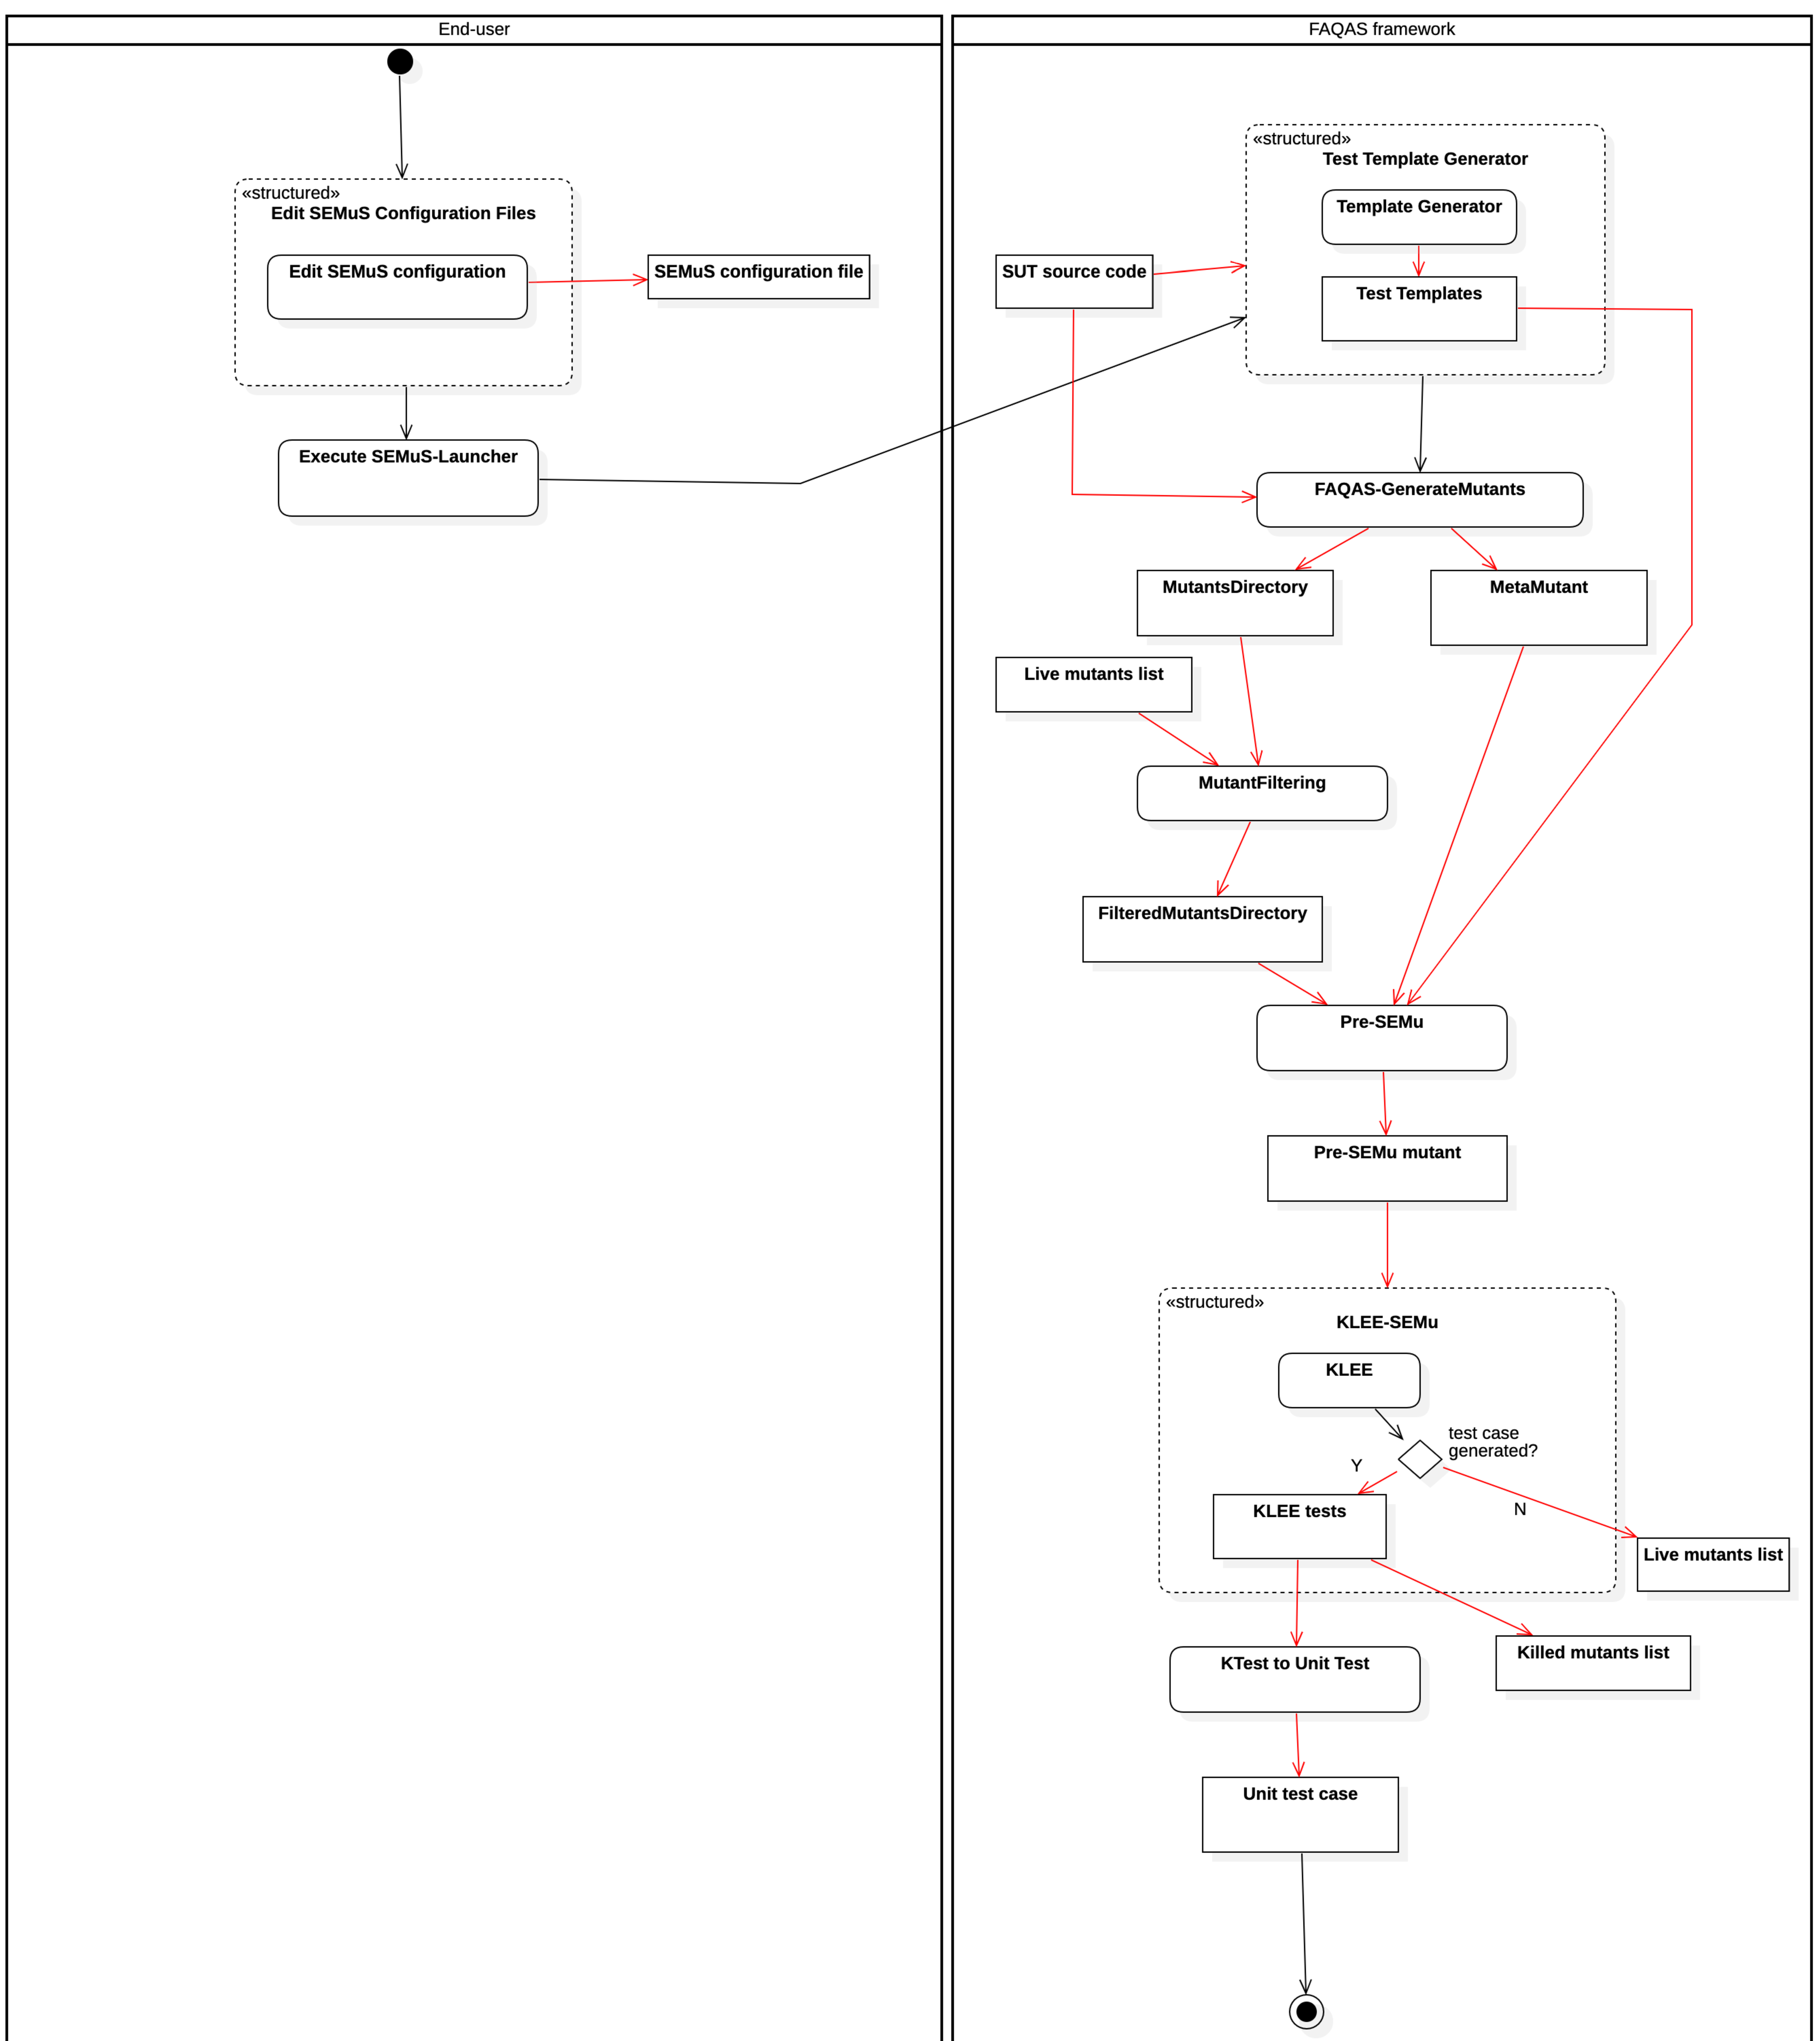
\includegraphics[width=\textwidth]{images/semus-activity.pdf}
      \caption{Overview of the code-driven test suite augmentation process.}
      \label{fig:process:codeDriven:augmentation}
\end{figure}

SEMuS implements the process for the improvement of the effectiveness of test suites, drafted in Figure~\ref{fig:process:codeDriven:augmentation}. Figure~\ref{fig:process:codeDriven:augmentation} relies on UML activity diagram notation. 
In Figure~\ref{fig:process:codeDriven:augmentation} the execution of specific software artefacts from the end user is made explicit. Also, we use black arrows to draw control-flow, red arrows for data-flow. The activities within the FAQAS Framework swimlane are implemented by a program (i.e., a Python or Bash script) that automates the activity. In the following we introduce a detailed description of the test suite augmentation process.

The activity \emph{Edit SEMuS Configuration} indicates that the engineers must configure the general configuration file; the end-user shall specify the SUT location, source code to be analyzed, and SEMu's specific configurations.

The activity \emph{Template Generator} indicates that SEMuS shall generate the \emph{TestTemplates} based on the SUT source code.
The content of file \emph{TestTemplates} should resemble \emph{Listing 1.23} of D2, it should enable the analysis with KLEE-SEMu. For example, it should have a call to the function targeted by the mutation. Also, it should contain the definition of all the variables used for the execution of KLEE-SEMu and a set of logging functions (e.g., \texttt{printf}) for the returned variable values.

The activity \emph{FAQAS-GenerateMutants} automatically generates a number of copies of each source file, the \emph{MutantsDirectory}, each copy contains one mutant. Additionally to the set mutant's sources, the component generates the \emph{MetaMutant}, which is a C file that embeds all the mutation into one single source file. More details of this activity can be found on Section~\ref{sec:behavior_mass}. 

The activity \emph{MutantFiltering} concerns the filtering of mutants for the test generation process; every mutant that is not present in the list of live mutants is removed from the analysis, and from the \emph{MutantsDirectory}. 

The activity \emph{Pre-SEMu} concerns the generation of a \emph{Pre-SEMu mutant}, that is, a compiled \emph{MetaMutant} file that includes the \emph{TestTemplate} for a specific function under analysis.

The activity \emph{KLEE-SEMu} indicates that SEMuS shall invoke KLEE-SEMu using the \emph{Pre-SEMu mutant} as input, to generate a tentative test input that kills the mutant under analysis. If KLEE-SEMu is not able to generate test inputs for the mutant it will add the identifier of the mutant to a list of live mutants, otherwise the test inputs are stored in the form of KLEE tests and the identifier of the mutant is added to a list of killed mutants.

The activity \emph{KTest To Unit Test} indicates that SEMuS collects the \emph{KLEE tests} generated by \emph{KLEE-SEMu} and generates a readable C unit test case. The test case generated by \emph{KTest to Unit Test} contains an invocation of the function under test (i.e., the function targeted  by the mutation) along with assigned arguments and an assertion that verifies results. The values for the assigned arguments and the verification of results are derived from the output of KLEE.

% The program \emph{FAQAS-GenerateTestGenerationScaffolding} takes as input the path of the \emph{SUT source code} and the file \emph{mutation results csv}. It generates a number of files named \emph{MutantId\_AnalysisMain.c}, one for each live mutant, where MutantId is the ID of a mutant. The file \emph{MutantId\_AnalysisMain.c} contains a main function that should be used for the analysis with KLEE. 



% The activity \emph{Update scaffolding for mutant} in Figure~\ref{fig:process:codeDriven:augmentation} indicates that the engineer should modify the file  \emph{MutantId\_AnalysisMain.c} if necessary. In particular, it might be necessary to refine the assertions produced by \emph{FAQAS-GenerateTestGenerationScaffolding}. More precisely, since assertions should concern output variables, it is necessary to verify that all the necessary output variables had been referred in assertion. Indeed, in C, with pointers and pointers to pointers, it is not possible to have a precise automated identification of output variables.

% The activities in the expansion region \emph{generateTestCase} are repeated for every live mutant.

% The activity \emph{Execute FAQAS-GenerateTestCase} in Figure~\ref{fig:process:codeDriven:augmentation} concerns the execution of the program \emph{FAQAS-GenerateTestCase}.

% The program \emph{FAQAS-GenerateTestCase} generates a tentative unit test case (i.e., a source file in C) that kills the mutant. It executes the KLEE program and then produces a unit test case (i.e., a file with a main in C) after processing the KLEE output.

% For test generation, the support for the programming language of the SUT depends on KLEE (it supports C, limited support for C++).

% The test case generated by \emph{FAQAS-GenerateTestCase} contains an invocation of the function under test (i.e., the function targeted  by the mutation) along with assigned arguments and an assertion that verifies results. The values for the assigned arguments and the verification of results are derived from the output of KLEE.

% If the program \emph{FAQAS-GenerateTestCase} successfully generates a test case, the engineer proceeds with inspecting it (activity \emph{Update Test  Case}), otherwise he can consider the mutant as equivalent (activity \emph{Update mutation results}).

% The activity \emph{Update Test  Case} in Figure~\ref{fig:process:codeDriven:augmentation} is performed by the engineer. He may need to execute the generated test case to verify that KLEE has generated valid inputs (e.g., inputs that meet the program preconditions). Based on KLEE results, \emph{FAQAS-GenerateTestCase} also generates assertions that reflect the output observed by KLEE (e.g., \texttt{assert( output == value\_observed\_by\_KLEE)} ). The engineer should thus also verify that the assertion with the expected value is correct (i.e., it reflects what indicated in the SUT specifications). If the value appearing in the assertion is not correct, it means that KLEE during its execution has observed an incorrect value being generated by the SUT; for this reason, the SUT might be faulty and should be fixed.

% The activity \emph{Add Test Case to SUT Test Suite} in Figure~\ref{fig:process:codeDriven:augmentation} is performed by the engineer, who may add the new test case to the test suite.

% The activity \emph{Update mutation results} in Figure~\ref{fig:process:codeDriven:augmentation} is performed when a test case is not generated. This generally happens when the mutant cannot be killed (i.e., is equivalent). The engineer is expected to manually inspect the mutant to be sure that the mutant is equivalent (otherwise the missing test case is due to a limitation of KLEE). If the mutant is equivalent the engineer removes it from the file \emph{mutation results csv}.

% The activity \emph{Execute FAQAS-RecomputeMutationScore} in Figure~\ref{fig:process:codeDriven:augmentation}  concerns the execution of the program \emph{FAQAS-RecomputeMutationScore}. It is performed after generating test cases for all the live mutants. Program \emph{FAQAS-RecomputeMutationScore} recomputes the mutation score after ignoring the equivalent mutants detected by KLEE.

\subsection{Internal interface design}

All the programs that automate the different steps of SEMuS communicate only through the files that had been described in Section~\ref{sec:component:design:semus}

\subsection{External interface design}

The external interfaces of the SEMuS are the programs that automate the different steps of SEMuS, which have been described above. They are:

\begin{itemize}
  \item \texttt{create\_mutants.sh}: launcher for the generation of mutants.
  \item \texttt{run.sh}: launcher for the generation of test inputs.
  \item \texttt{docker\_run.sh}: launcher for the generation of test inputs by means of Docker.
\end{itemize}







